\documentclass{beamer}
\setbeamertemplate{navigation symbols}{}

\usepackage{beamerthemeshadow}
\setbeamertemplate{caption}[numbered]

\hypersetup{colorlinks}

\def\gw#1{gravitational wave#1 (GW#1)\gdef\gw{GW}}
\def\ns#1{neutron star#1 (NS#1)\gdef\ns{NS}}

\newcommand{\red}[1]{{\color{red}{#1}}}

\begin{document}
\title{NS Group Update}
\subtitle{Burst Call Jan 21$^{\text{st}}$ 2015}  
\author{James A. Clark (for the NS group)}
\institute{Georgia Institute Of Technology}
\date{} 

\begin{frame}[plain]
\titlepage
\end{frame}

\begin{frame}\frametitle{Table of contents}\tableofcontents
\end{frame} 

\section{NS Group}

\begin{frame}
    \frametitle{The Group}
    Joining the group:
    \begin{itemize}
        \item Calls: bi-weekly, Friday 11am EST, burst TeamSpeak channel
        \item
            {\small\href{https://wiki.ligo.org/viewauth/GIANT/GIANTteleconAgendas}
            {https://wiki.ligo.org/viewauth/GIANT/GIANTteleconAgendas}}
        %\item Call time negotiable!
        %\item External speakers to resume soon, watch this space\dots
    \end{itemize}
    Scope:
    \begin{itemize}
        \item Explore / discuss astrophysics \& data analysis strategies
            pertaining to transient, unmodelled \gw{} bursts from \ns{s}
    \end{itemize}
    Projects:
    \begin{itemize}
        \item Long bursts: Proto-magnetar deformations \& Magnetar QPOs
        \item Short bursts: Post-BNS \& magnetars
        \item \dots others welcome!
    \end{itemize}
\end{frame}

\section{NS Search Proposal}

\begin{frame}
    \frametitle{NS Search Proposal}
    Search proposal wrapped up and reviewer responses addressed:
    \begin{itemize}
        \item Current draft in DCC: {\small \href{https://dcc.ligo.org/LIGO-T1400606}{https://dcc.ligo.org/LIGO-T1400606}}
        \item Reviewer comments / responses: \url{https://wiki.ligo.org/DAC/NS}
    \end{itemize}
    For O1 plan is to only target \emph{extraordinary} events:
    \begin{itemize}
        \item Hyper-flares from Galactic magnetars (c.f., SGR 1806-20):
            X-pipeline \& STAMP
        \item BNS: long bursts (STAMP / X-pipeline) from long-lived remnant,
            short bursts from short- or long-lived post-merger remnant
    \end{itemize}
    Review comments addressed, only substantive change: short post-merger
    analysis to be PE-style follow-up, not a search.
\end{frame}

\section{Project News}

\subsection{BNS Long Bursts}
\begin{frame}
    \frametitle{BNS Long Burst Study}
    Preliminary MDC study to assess sensitivity to long-duration, slightly
    non-stationary signals from stable BNS remnants
    \begin{itemize}
        \item People: Michael Coughlin, Scott Coughlin, James Clark, Ryan
            Quitzow-James, Marie-Anne Bizourd, Nelson Christensen, Patrick
            Meyers, Eric Thrane
        \item Basic idea: BNS merger \emph{may} result in a long-lived, massive
            neutron star; $B$-fields could result in quadrupole deformation
            (e.g., \url{http://arxiv.org/abs/1408.0013})
        \item Signal: anti-chirp starting $\sim$kHz sweeps down in frequency
            over $\mathcal{O}(10^6)$\,s
        \item Optimal search: 10--100\,Mpc / 0.1--1 year$^{-1}$
    \end{itemize}
\end{frame}

\begin{frame}
    \frametitle{BNS Long Burst Study}
    As a preliminary MDC study, considering slowly varying ($\dot{f}<0$) signals
    at 600, 750 \& 900\,Hz with $\tau\sim250$\,s.\\~\\

    Goals:
    \begin{itemize}
        \item Deploy simulation infrastructure appropriate for long signals:
            using swig-wrapped LAL routines in python module
        \item Using a week of S6 data as playground (GPS 946086263--946691063)
        \item Target common set of MDC frames using X-pipeline \& STAMP
        \item Will consider more physical (longer duration) signals later once
            infrastructure and comparisons are in place
    \end{itemize}

\end{frame}

\begin{frame}
    \frametitle{BNS Long Burst Study: Example STAMP Recovery}
    \begin{figure}
        \centering
        \scalebox{0.3}{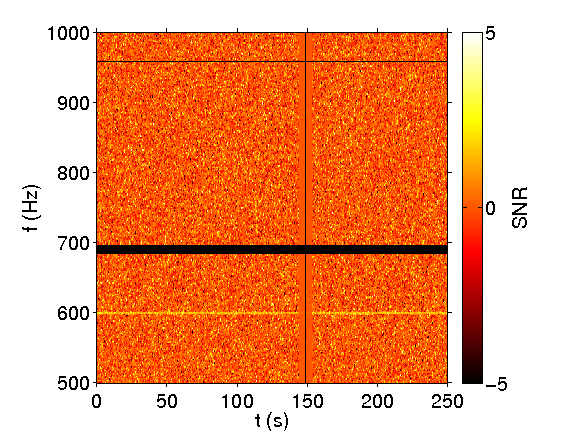
\includegraphics{example_snr_map_stamp.png}}
    \end{figure}
\end{frame}

\begin{frame}
    \frametitle{BNS Long Burst Study: \emph{Preliminary} STAMP Results}
    \begin{itemize}
        \item Use a background threshold corresponding to $\sim1/10^4$ maps
        \item $50\%$ FAP sensitivity (network) SNRs of
            \begin{itemize}
                \item $f_0=600$\,Hz: $\rho_{\rm{net}}=33$
                \item $f_0=900$\,Hz: $\rho_{\rm{net}}=33$
            \end{itemize}
        \item Sensitivities seem reasonable for waveform duration and nature of
            clustering
    \end{itemize}
    Summary:
    \begin{itemize}
        \item Simulation infrastructure in place to inject \& recover long,
            multi-frame signals in noise, common to multiple
            analyses\footnote{modulo a potential timing bug which should now be
            resolved}
        \item Some preliminary sensitivity estimates for toy model
        \item Next: extent and explore toy models/parameters, investigate longer
            signals
    \end{itemize}

\end{frame}

\subsection{Post-BNS Short Bursts}
%\begin{frame}
%    \tableofcontents[currentsection,currentsubsection]
%\end{frame}

\begin{frame}
    \frametitle{Post-BNS Short Bursts}
    Search plan also calls for BNS follow-ups targeting short, high-freq burst
    immediately after merger via (e.g.):
    \begin{itemize}
        \item Coherent WaveBurst: post-merger analysis via reconstructed
            time-freq map / PSD of reconstructed signal (similar to previous work)
        \item LALInference Burst (LIB): `vanilla' LIB searches with sine-Gaussian
            templates, given a narrow time prior and returns (e.g.) signal/noise
            evidence, amplitude \& frequency posteriors
        \item BayesWave: similar post-merger analysis to CWB
    \end{itemize}
    Some preliminary results from LIB \& CWB analyses in-hand
\end{frame}

\begin{frame}
    \frametitle{LIB Studies}
    \begin{itemize}
        \item Some development / debugging was required to get end-to-end LIB
            analysis of on-the-fly NINJA-style injections (no MDC frame
            generation necessary)\footnote{successful NINJA injections in LIB
            will also be useful for SNe}
        \item Have a test run of $100$ post-merger injections
            \url{https://ldas-jobs.ligo-wa.caltech.edu/~jclark/LIB/pmns/shen_135135/lib_3.6-Mpc}
        \item Results consistent with past LIB experience: tendency for
            frequency posterior to lock on to low-frequency content from
            inspiral/merger \& miss the post-merger signal
    \end{itemize}
\end{frame}

%\begin{frame}
%    \frametitle{LIB Studies}


\begin{frame}
    \frametitle{CWB Studies}
    Also looking at CWB reconstructions\footnote{piggy-backing on McIver's SN
    reconstruction studies} via CEDs of post-merger injections\\~\\
    Motivations:
    \begin{itemize}
        \item Standard LIB alone prone to mis-identifying the interesting part
            of the signal
        \item Determine post-merger reconstruction fidelity, especially recovery
            of high frequencies
        \item Side project: how well can we determine inspiral/merger peak time?
            May be useful for guiding the LIB follow-up \& interesting to
            compare CWB reconstructed peak time with CBC template's
            time-of-coalescence
    \end{itemize}
\end{frame}

\begin{frame}
    \frametitle{CWB CED Example}
    Handful of example CEDs (for 3.6\,Mpc injections):
    {\tiny
    \url{https://ldas-jobs.ligo.caltech.edu/~jlmciver/reports/ADV_SIM_PMNS_SHEN135135_MR/ced/}}

    \begin{columns}[]
        \column{0.5\textwidth}
        \begin{center}
        \begin{figure}
            \vspace*{-0.5cm}
    %        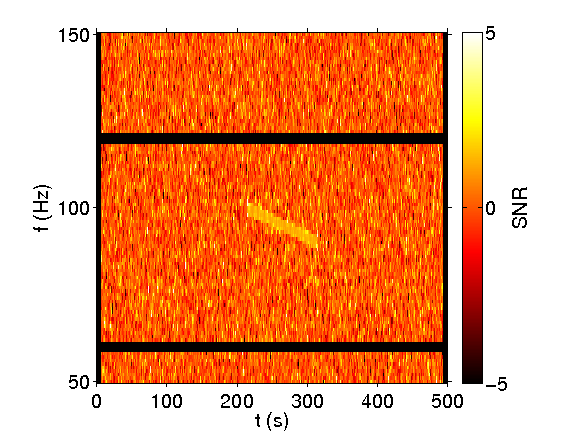
\includegraphics[scale=0.3]{qpo_tf.png} 
        \end{figure}
        \end{center}

        \column{0.5\textwidth}
        \begin{center}
        \begin{figure}
            \vspace*{-0.5cm}
    %        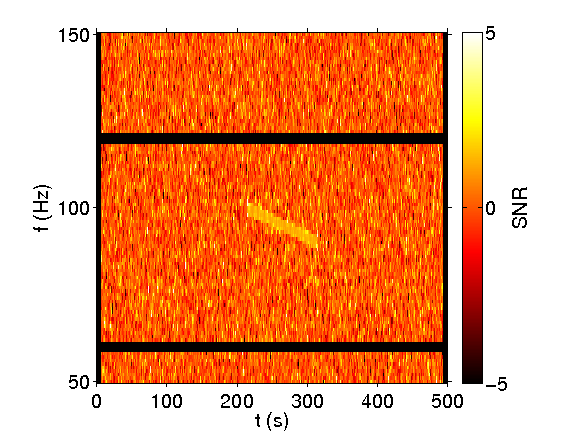
\includegraphics[scale=0.3]{qpo_tf.png} 
        \end{figure}
        \end{center}
    \end{columns}
    Similar issues to LIB: high-frequency component is not robustly detected /
    recovered; improvements may be possible with clustering (TBD)

\end{frame}


\begin{frame}
    \frametitle{Summary}
    {\small 
    Group now quite active in addressing studies for follow-ups of extraordinary
    events in O1 (and beyond!)
    \begin{itemize}
        \item Infrastructure $\sim$in place for making MDC frames
            for common post-BNS long burst STAMP and X-pipeline studies
        \item Preliminary STAMP results for toy model post-BNS long bursts in
            hand and in line with expectation
        \item Similar simulation infrastructure checking / development for
            post-BNS short bursts
        \item Prelim. LIB results for on-the-fly NINJA injections of short
            BNS bursts
        \item Prelim. Multi-res CWB 2G results for similar NINJA injections (via
            MDC frames but same functions as LIB)
    \end{itemize}
    Coming weeks: scale up all studies \& develop necessary
    modifications/refinements to configurations and searches to better target
    astrophysical results
}

\end{frame}




\end{document}
